\documentclass[11pt,a4paper]{article}
\usepackage[margin=28mm]{geometry}
\usepackage{fontspec}
\usepackage{xcolor}
\usepackage{graphicx}
\usepackage{tikz}
\usepackage{hyperref}
\setmainfont{Latin Modern Roman}
\definecolor{forest}{HTML}{2F5144}
\hypersetup{colorlinks=true,urlcolor=forest}
\title{\color{forest}\Huge The art of a\\well-made document}
\author{A little space for big ideas}
\date{\today}

\begin{document}
\maketitle
\thispagestyle{empty}

\begin{abstract}
Every great idea deserves a beautiful page. This is your
space to think clearly, write freely, and bring something
worth reading into the world.
\end{abstract}

\section{Begin with an idea}
A blank page is an invitation. Whether you are writing a
research paper, preparing a lesson, or exploring a new
thought, good typography lets your ideas take the lead.

PaperStudio brings your words, mathematics, and images
together in one considered workspace.

\section{Make room for discovery}
Some ideas are best expressed in the language of mathematics:
\begin{equation}
  e^{i\pi} + 1 = 0
\end{equation}
Others need a picture. With TikZ, even a simple diagram
can tell a story.

\begin{center}
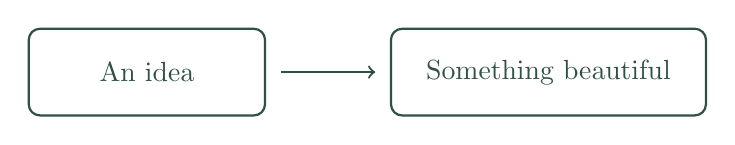
\begin{tikzpicture}
  \draw[forest, thick, rounded corners=4pt]
    (0,0) rectangle (3,1.1);
  \node[text=forest] at (1.5,.55) {An idea};
  \draw[->, thick, forest] (3.2,.55) -- (4.4,.55);
  \draw[forest, thick, rounded corners=4pt]
    (4.6,0) rectangle (8.6,1.1);
  \node[text=forest] at (6.6,.55) {Something beautiful};
\end{tikzpicture}
\end{center}

\section{Your next chapter}
This is only the beginning. Try the Sinhala template,
upload an image, or make this document your own.
\end{document}
